% Options for packages loaded elsewhere
\PassOptionsToPackage{unicode}{hyperref}
\PassOptionsToPackage{hyphens}{url}
%
\documentclass[
  12pt,
]{article}
\usepackage{lmodern}
\usepackage{amssymb,amsmath}
\usepackage{ifxetex,ifluatex}
\ifnum 0\ifxetex 1\fi\ifluatex 1\fi=0 % if pdftex
  \usepackage[T1]{fontenc}
  \usepackage[utf8]{inputenc}
  \usepackage{textcomp} % provide euro and other symbols
\else % if luatex or xetex
  \usepackage{unicode-math}
  \defaultfontfeatures{Scale=MatchLowercase}
  \defaultfontfeatures[\rmfamily]{Ligatures=TeX,Scale=1}
  \setmainfont[]{Times New Roman}
\fi
% Use upquote if available, for straight quotes in verbatim environments
\IfFileExists{upquote.sty}{\usepackage{upquote}}{}
\IfFileExists{microtype.sty}{% use microtype if available
  \usepackage[]{microtype}
  \UseMicrotypeSet[protrusion]{basicmath} % disable protrusion for tt fonts
}{}
\makeatletter
\@ifundefined{KOMAClassName}{% if non-KOMA class
  \IfFileExists{parskip.sty}{%
    \usepackage{parskip}
  }{% else
    \setlength{\parindent}{0pt}
    \setlength{\parskip}{6pt plus 2pt minus 1pt}}
}{% if KOMA class
  \KOMAoptions{parskip=half}}
\makeatother
\usepackage{xcolor}
\IfFileExists{xurl.sty}{\usepackage{xurl}}{} % add URL line breaks if available
\IfFileExists{bookmark.sty}{\usepackage{bookmark}}{\usepackage{hyperref}}
\hypersetup{
  pdftitle={Is big tech greenwashing?},
  pdfauthor={Amanda Booth and Ricky Prophete},
  hidelinks,
  pdfcreator={LaTeX via pandoc}}
\urlstyle{same} % disable monospaced font for URLs
\usepackage[margin=2.54cm]{geometry}
\usepackage{longtable,booktabs}
% Correct order of tables after \paragraph or \subparagraph
\usepackage{etoolbox}
\makeatletter
\patchcmd\longtable{\par}{\if@noskipsec\mbox{}\fi\par}{}{}
\makeatother
% Allow footnotes in longtable head/foot
\IfFileExists{footnotehyper.sty}{\usepackage{footnotehyper}}{\usepackage{footnote}}
\makesavenoteenv{longtable}
\usepackage{graphicx,grffile}
\makeatletter
\def\maxwidth{\ifdim\Gin@nat@width>\linewidth\linewidth\else\Gin@nat@width\fi}
\def\maxheight{\ifdim\Gin@nat@height>\textheight\textheight\else\Gin@nat@height\fi}
\makeatother
% Scale images if necessary, so that they will not overflow the page
% margins by default, and it is still possible to overwrite the defaults
% using explicit options in \includegraphics[width, height, ...]{}
\setkeys{Gin}{width=\maxwidth,height=\maxheight,keepaspectratio}
% Set default figure placement to htbp
\makeatletter
\def\fps@figure{htbp}
\makeatother
\setlength{\emergencystretch}{3em} % prevent overfull lines
\providecommand{\tightlist}{%
  \setlength{\itemsep}{0pt}\setlength{\parskip}{0pt}}
\setcounter{secnumdepth}{5}

\title{Is big tech greenwashing?}
\usepackage{etoolbox}
\makeatletter
\providecommand{\subtitle}[1]{% add subtitle to \maketitle
  \apptocmd{\@title}{\par {\large #1 \par}}{}{}
}
\makeatother
\subtitle{\url{https://github.com/amandafbooth/BoothProphete_ENV872_EDA_FinalProject}}
\author{Amanda Booth and Ricky Prophete}
\date{}

\begin{document}
\maketitle

\newpage
\tableofcontents 
\listoftables 
\listoffigures 
\newpage

\hypertarget{rationale-and-research-questions}{%
\section{Rationale and Research
Questions}\label{rationale-and-research-questions}}

As the world searches for climate change mitigation strategies in the
face of apocalyptic climate projections and escalating real-world
effects, the need to decarbonize the global economy has placed
increasing societal and political pressure on companies to limit their
emissions. Part of this pressure has come from the Environmental,
Social, and Governance investing movement, which focuses on
sustainability as a key part of identifying material risks and growth
opportunities for companies.

Corporations have responded to the decarbonization challenge posed by
these external forces by self-disclosing their carbon footprints along
with action plans for reducing them over a specified time horizon.
However, there are 2 key issues with the self-disclosure model:

\begin{itemize}
\item
  Current emissions accounting and reporting practices have not been
  harmonized, leading to differential approaches to carbon accounting.
\item
  Given a lack of oversight in emissions reporting and the nature of
  informational asymmetries between organizations and investors,
  companies face perverse incentives to understate their carbon
  footprint and/or otherwise mischaracterize their progress toward
  decarbonization.
\end{itemize}

There have been recent efforts to address these issues. In March of
2022, the Securities and Exchange Commission (SEC) proposed rule
amendments that would require companies to incorporate specific
climate-related information in their statements and reports. This rule
would also impose additional disclosure requirements on organizations
that have made public commitments to take steps to address climate
change. As part of their rationale for the proposed rule changes, the
SEC noted both the need to harmonize disclosure standards and a desire
to mitigate attempts by companies to engage in ``green-washing'' or
``climate-washing''.

It is in this context that we sought to understand the extent to which
companies might be engaged in green- or climate-washing, and whether
organizations engaged in these behaviors possessed specific attributes
that could reliably predict the propensity of such behavior. To
investigate this, we reviewed a partial dataset from the Carbon
Disclosure Project (CDP), which is a nonprofit that manages a global
carbon emissions disclosure system. As CDP data is paywalled, we were
able to access this partial dataset via a study published in Nature
(Klaaßen \& Stoll). This dataset and its attributes are described in
greater detail in our Dataset Information section.

Our primary research question was the following:

\begin{itemize}
\tightlist
\item
  What attributes are the strongest predictors for emissions reporting
  discrepancies?
\end{itemize}

Over the course of our work, our dataset inspired an additional
question:

\begin{itemize}
\tightlist
\item
  What attributes are the strongest predictors for an organization's
  total energy consumption?
\end{itemize}

\newpage

\hypertarget{dataset-information}{%
\section{Dataset Information}\label{dataset-information}}

\hypertarget{data-retrieval}{%
\subsection{Data Retrieval}\label{data-retrieval}}

For this analysis, we used data analyzed in a \emph{Nature
Communications} study that took data from 2019 CDP reports. CDP, a
carbon footprint registry for companies and municipalities, conducts an
in-depth questionnaire that inquires about the details of what entities
do and don't include in their carbon emissions reporting. The
\emph{Nature} study compared what technology companies published in
their official company reports to what companies reported in CDP
questionnaires and found technology companies often under reported
emissions in official company reports. The data from nature came in the
form of an Excel Workbook with many panels. We converted three panels
into CSVs for analysis in R:

\begin{itemize}
\tightlist
\item
  Company information
\item
  Emissions predictors
\item
  Reporting inconsistencies
\end{itemize}

Table 1: Data Information

\begin{longtable}[]{@{}ll@{}}
\toprule
\begin{minipage}[b]{0.58\columnwidth}\raggedright
\textbf{Detail}\strut
\end{minipage} & \begin{minipage}[b]{0.36\columnwidth}\raggedright
\textbf{Description}\strut
\end{minipage}\tabularnewline
\midrule
\endhead
\begin{minipage}[t]{0.58\columnwidth}\raggedright
Data Source\strut
\end{minipage} & \begin{minipage}[t]{0.36\columnwidth}\raggedright
Nature Communications\strut
\end{minipage}\tabularnewline
\begin{minipage}[t]{0.58\columnwidth}\raggedright
Retrieved from\strut
\end{minipage} & \begin{minipage}[t]{0.36\columnwidth}\raggedright
\url{https://www.nature.com/articles/s41467-021-26349-x}\strut
\end{minipage}\tabularnewline
\begin{minipage}[t]{0.58\columnwidth}\raggedright
Variables Used\strut
\end{minipage} & \begin{minipage}[t]{0.36\columnwidth}\raggedright
Company, Sales, Profits, Assets, Market value, Company report, CDP
emissions, Emission reports deviation, Reporting inconsistency ratio,
Total energy consumption\strut
\end{minipage}\tabularnewline
\begin{minipage}[t]{0.58\columnwidth}\raggedright
Data Collection Year\strut
\end{minipage} & \begin{minipage}[t]{0.36\columnwidth}\raggedright
2019\strut
\end{minipage}\tabularnewline
\bottomrule
\end{longtable}

\newpage

\hypertarget{exploratory-analysis}{%
\section{Exploratory Analysis}\label{exploratory-analysis}}

\begin{longtable}[]{@{}ll@{}}
\caption{Top 5 Companies by Highest Reporting Inconsistency
Ratio}\tabularnewline
\toprule
Company & Inconsistency\_ratio\tabularnewline
\midrule
\endfirsthead
\toprule
Company & Inconsistency\_ratio\tabularnewline
\midrule
\endhead
Samsung SDI & 0.9994994\tabularnewline
SAP & 0.9620065\tabularnewline
Adobe & 0.9005902\tabularnewline
Salesforce.com & 0.8326687\tabularnewline
IBM & 0.7553958\tabularnewline
\bottomrule
\end{longtable}

\newpage

\hypertarget{analysis}{%
\section{Analysis}\label{analysis}}

\hypertarget{question-1-insert-specific-question-here-and-add-additional-subsections-for-additional-questions-below-if-needed}{%
\subsection{Question 1: \textless insert specific question here and add
additional subsections for additional questions below, if
needed\textgreater{}}\label{question-1-insert-specific-question-here-and-add-additional-subsections-for-additional-questions-below-if-needed}}

\hypertarget{question-2}{%
\subsection{Question 2:}\label{question-2}}

\newpage

\hypertarget{summary-and-conclusions}{%
\section{Summary and Conclusions}\label{summary-and-conclusions}}

We did not find a statistically significant relationship between
companies' reporting discrepancy ratios and variables that indicate
size. As expected, we found a relationship between total energy
consumption and size indicators. But surprisingly the indicator with the
most confidence was value of assets.

\begin{figure}
\centering
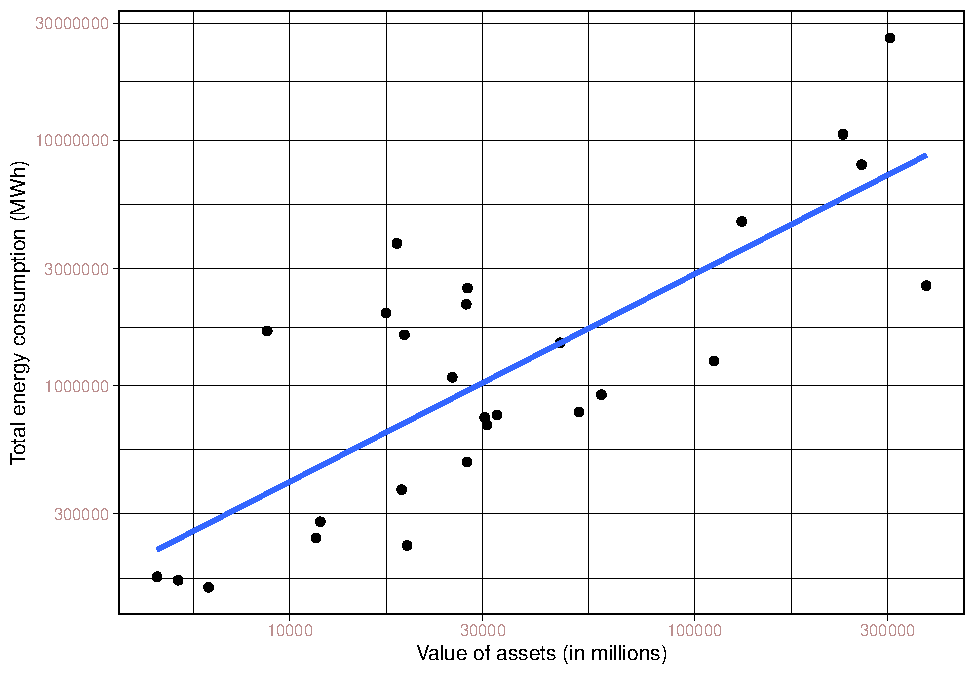
\includegraphics{BoothProphete_Report_files/figure-latex/plot1-1.pdf}
\caption{Relationship between asset value and total energy consumption}
\end{figure}

Our assumption that ``big tech'' would show more reporting discrepancies
was not borne out in the data we analyzed. In future analyses on this
topic, we would ideally have access to more CDP reports and more
corporate reports in order to have a sample size that allows for more
statistically accuracy.

\newpage

\hypertarget{references}{%
\section{References}\label{references}}

Klaaßen, Lena, and Christian Stoll. ``Harmonizing Corporate Carbon
Footprints.'' Nature News, Nature Publishing Group, 22 Oct.~2021,
\url{https://www.nature.com/articles/s41467-021-26349-x}.

\end{document}
